\documentclass[output=paper]{LSP/langsci} 
\author{Nomi Erteschik-Shir	\affiliation{Ben Gurion University}\lastand 
	Gunlög Josefsson\affiliation{Lund University}
}
\title{Scandinavian object shift is phonology} 
% \epigram{Change epigram}
\abstract{The problem addressed in this paper is a case of word order microvariation in Mainland Scandinavian: optional vs. obligatory Object Shift (OS). Following standard assumptions (see \citealt{Selkirk1996}), weak object pronouns are assumed to be affixal clitics at PF which do not themselves have the status of prosodic words. Since adverbs (including negation), are unsuitable as hosts, weak object pronouns may undergo OS, in other words precede adverbs, ending up encliticized onto the preceding verb or subject. In standard Danish, OS is obligatory; the order adverb+weak pronoun is blocked. However, in Swedish, OS is optional, as is the case for some Danish dialects, spoken in the southeastern island area. In our paper we explain the distribution of optional vs. obligatory OS by the phonological properties of the two varieties. What “optional OS” in Swedish and varieties of Danish have in common is the occurrence of a tonal accent, which creates a larger phonological unit than the minimal prosodic word, a Tonal Unit. We propose that the mechanism that allows a weak pronoun to remain in the canonical position in Swedish and the southeastern island dialects in Danish, is the availability of tonal accent. The tonal accent enables the inclusion of the pronoun in such a unit. Standard Danish, on the other hand, lacks tonal accent altogether which is why OS is obligatory in this dialect.
}

\ChapterDOI{10.5281/zenodo.1117700}
\maketitle

\begin{document}
\section{Introduction} 
Since \citealt{Holmberg1986}, pronominal object shift, OS, in the \ili{Mainland Scandinavian} languages, henceforth MSc, has become a widely studied and carefully described phenomenon. It refers to the placement of a weak object pronoun to the left of a sentence adverb, such as the \isi{negation}, \REF{ex:erteschik:1a}, instead of in the canonical position for objects, which is to the right of a sentence adverb, \REF{ex:erteschik:1b}.  

\noindent\parbox{\textwidth}{\ea \ili{Swedish}\\%1
    \label{ex:erteschik:1}
\ea  \label{ex:erteschik:1a}

    \gll Jag   mötte   honom   inte.\\
	   I    met    him    not\\
    \glt      ‘I didn’t meet him.’

\ex  \label{ex:erteschik:1b}
\gll Jag   mötte   inte   honom.   \\
    I    met    not  him\\
\glt
       ‘I didn’t meet him.’
\z
\z}

Following standard assumptions (see \citealt{Selkirk1996}), we assume that weak object pronouns are affixal clitics at PF which do not themselves have the status of prosodic words, and that this holds generally for OS in MSc. Whether or not OS is obligatory, however, varies among the MSc languages and varieties. In this article we will concentrate on \ili{Danish} and \ili{Swedish}. However, we are convinced that the ideas proposed here can be applied more generally in MSc. Somewhat simplified, OS is obligatory in most \ili{Danish} dialects, except for certain areas in southern Denmark (for example the dialect spoken on the {island} of Ærø), where OS is optional. In \ili{Swedish} OS is optional, except for \ili{Fenno-Swedish} and \ili{Oevdalian} \ili{Swedish}.\footnote{It should be pointed out that our study is restricted to pronominal shift in the \ili{Mainland Scandinavian} languages. Naturally, it  would be interesting to explore to what extent our findings could be applied to full DP shift, as in \ili{Icelandic}, but that {question} will not be explored in this article.} 

In this paper we demonstrate that optionality of OS in MSc is conditioned by language- and variety-specific phonological properties, and thus PF is responsible for at least some microvariation in word order. Our argument however goes further: We claim, following  \citealt{Erteschik-Shir2005Sound} and \citealt{Josefsson2010,Josefsson2012}, that OS in the \ili{Mainland Scandinavian} languages is in fact driven by phonology. The basis of our claim is the well-known requirement of weak pronouns to incorporate, and thus to form a prosodic unit with a legitimate host. In the shifted word order, the host is the preceding verbal or nominal element. This is shown in the \ili{Danish} examples below.\footnote{Similar examples could be drawn from the other MSc dialects, except for \ili{Fenno-Swedish}, discussed in \sectref{sec:erteschik:5}.}

\ea \label{ex:erteschik:2}%2
    \ili{Danish}\\ 
\ea 
\gll Jeg {mødte ham}   ikke. \\
          I      met=him     not\\
    \glt  ‘I didn’t meet him.' 

\ex 
\gll Hvorfor   mødte   {Peter ham}     ikke.\\
why        met       Peter=him     not\\
        \glt  ‘Why didn’t Peter meet him.'
\z
\z

At first glance it could be tempting to explain the variation by assuming a word order parameter that would determine whether adverbs may be hosts or not.\footnote{Negation behaves like other adverbs in \ili{Scandinavian} and is therefore classified as an adverb here.} However, such a solution would be a simple reformulation of the empirical observation, thus circular and devoid of explanatory {force}. Therefore, we will hold on to the generalization that adverbs in general are not legitimate hosts for prosodic incorporation or \isi{cliticization}, thus that weak pronouns cannot cliticize onto adverbs in any of the MSc varieties.\footnote{Languages vary as to which elements can host prosodic incorporation or \isi{cliticization}. In \ili{Scandinavian} languages, for example, but not in English, nominals can host these processes. We do not expect to find adjoined modifiers, such as adverbs as hosts crosslinguistically. In the cases we discuss here, the formation of the prosodic unit between the adverb and the weak pronoun is due to the tonal accent, not to the capability of the adverb to be a host for incorporation.}  Instead, we argue that the varieties that allow optional OS – varieties where the weak object pronoun may follow an adverb as in \REF{ex:erteschik:1b} – offer another possibility of  prosodic incorporation, namely a prosodic unit created by (the presence of) tonal accent. (This will be elaborated in \sectref{sec:erteschik:4}.)

The idea that prosodic factors determine OS is important more generally, since it shows that PF can be responsible for microvariation in word order. If this is the case, the claim that word order is entirely determined by syntax is put into {question}.

\section{Previous proposals on OS, phonology, and information structure}\label{sec:erteschik:2}

The idea that OS has phonological properties has been suggested in the literature. More specifically it has been proposed that weak object pronouns are clitics or clitic-like elements (see \citealt[167]{Holmberg1991}; \citealt{Josefsson1992,Josefsson1993,Josefsson1994,Josefsson2010,Josefsson2012}; \citealt[122]{Déprez1994}; \citealt{Hellan1994,Hellan2005}; \citealt[207]{BobaljikJonas1996}; \citealt[77]{Diesing1996kluwer}; \citealt[41]{Diesing1997}; \citealt{Erteschik-Shir2005Sound,Erteschik-Shir2005WhatIs,Hosono2010,Hosono2013}). 

The fact that stressed pronouns cannot undergo OS inspired \citet[25–28]{Holmberg1999} to propose that OS is driven by a formal feature related to information structure. Holmberg suggests that objects that undergo OS are marked [-\isi{Focus}], and that they need to be c-commanded by a category marked  [+\isi{Focus}]. The reason shift never takes place across verbs, verb particles, or prepositions (for Holmberg’s Generalization, see \citealt{Holmberg1986,Holmberg1999}) would be that such categories are inherently marked [-\isi{Focus}], which means that there would be no trigger for movement of the object to a higher position.  Adverbs, on the other hand, are not marked [-\isi{Focus}] in this framework, which would explain why they do not block OS. The requirement that a [-\isi{Focus}] element has to be licensed by a [+\isi{Focus}] element would, in fact, be what forces movement. A suggestion along the same lines was suggested in \citet{Platzack1996}, where a feature Repel F was introduced. The role of this feature is to {force} a [-\isi{Focus}] element, for example, to move out of a focus domain.

\section{Phonological background}\label{sec:erteschik:3}

Since our account is phonological in nature, a short introduction to the phonological theory  which we base our analysis on is called for. 

\subsection{ Stress and (minimal) prosodic words in MSc}\label{sec:erteschik:3.1}

Basing their claims on \ili{Swedish}, \citet{Myrberg2013}, see also \citet{Riad2013}, define a minimal prosodic word in terms of culminativity; a minimal prosodic word is a constituent with exactly one stress. Consequently, most simplex words and derivations are minimal prosodic words. A \isi{compound}, such as \textit{hus-båt} (house-boat) ‘house boat’ and certain derivations, for example \textit{tvätt-bar} (wash-BAR) ‘washable’, have two stresses, primary stress on the first constituent, and secondary stress on the second constituent, which means that they consist of two minimal prosodic words [ˈhʉːsˌboːt] and [ˈtvɛtˌbɑːr]. \isi{Compounds}\is{compound} and other prosodic words with two stresses are classified as maximal prosodic words. These are discussed in \sectref{sec:erteschik:3.2}.

  Following \citealt{Selkirk1996}, there is no one-to-one correspondence between prosodic and morphosyntactic words. For instance, the PP \textit{med bil} `with car’, as in \textit{Vi åkte med bil} `We went by car’, is pronounced as a minimal prosodic word: [məˈbiːl], and the unit has the same prosodic contour as e.g. the morphosyntactic word \textit{banan} ‘banana’: [baˈnɑːn]. In a similar way, weak object pronouns may incorporate into prosodic words. \citet[131]{Riad2013} exemplifies this with the verb \textit{gav} ‘gave’ [ˈɡɑːv], followed by the object pronoun \textit{henne} ‘her’ (pronounced [ˈhənə] in isolation), which may form a minimal prosodic word, [ˈɡɑːvənə] ‘gave her’. The loss of /h/ in this position indicates that the first syllable of \textit{henne} is neither stressed, nor initial in a prosodic word. (/h/only occurs initially in minimal prosodic words in \ili{Swedish}.) Furthermore, the syllabification is \textit{ga.ve.ne} (rather than *\textit{gav.e.ne}), which indicates a single syllabification domain, i.e. a single minimal prosodic word. 

  As we have seen, Riad discusses examples of verb + weak object pronouns. However, if we include weak subject pronouns in the discussion, we conclude that the formation of prosodic words does not depend on syntactic constituency. The sequence \textit{jag såg} ‘I saw’ [jaˈsoː] in \textit{jag såg hönor} ‘I saw chickens’ forms one prosodic word, distinct from the object \textit{hönor} `chickens’ [ˈhøːnər], which is a prosodic word by itself: [jaˈsoːˈhøːnər] – it is possible to make a break before \textit{hönor}.  Furthermore, it would be incorrect to leave the [h] sound out in this example, *[ˈøːnər], which is a strong indication that the object \textit{hönor} `chickens’ is a (minimal) prosodic word of its own in this case. Further support that \textit{hönor} `chickens’ in the example in {question} is a minimal prosodic word on its own is supported by the fact that it has Accent 2, as opposed to \textit{jag såg} `I saw’, which has Accent 1. Assuming that verb + object form a syntactic constituent, the subject + verb example shows that a prosodic word can consist of units that are not syntactic. 

  What will be important in the following is the assumption that weak object pronouns are pronouns that have to incorporate into a prosodic word. 

\subsection{Tonal accent and tonal units in Mainland Scandinavian}\label{sec:erteschik:3.2}

In addition to stress, most \ili{Swedish} and \ili{Norwegian} dialects, as well as some Southern \ili{Danish} dialects, distinguish two tonal accents:  Accent 1 and Accent 2. These accents may differentiate word pairs with two or more syllables in these languages. The actual \isi{tone} contour differs between dialects, but a typical Stockholm variant is shown below:

\ea%3
\label{ex:erteschik:3}
 Stockholm \ili{Swedish} (from \citealt[184]{Riad2013})\\
 \begin{tabular}[t]{lllllcc}
 & & & & &  word accent & focus accent\\
 anden & ‘the duck’  & [\textsuperscript{1}ˈandən]   & → & Accent 1 & HL*       &      L*H\\
 anden & ‘the ghost’ & [\textsuperscript{2}ˈandən]   & → & Accent 2 & H*L       &      H*LH\\ 
 \end{tabular}
\z

In Standard \ili{Swedish}, \isi{compounds}\is{compound} and words derived by suffixes generally have Accent 2:

\ea%4
\label{ex:erteschik:4}
\ea \label{ex:erteschik:4a} \textit{hus-båt} (house-boat) ‘houseboat’      [\textsuperscript{2}ˈhʉːsˌboːt]
\ex \label{ex:erteschik:4b} \textit{tvätt-bar} (wash-BAR) ‘washable’       [\textsuperscript{2}ˈtvɛtˌbɑːr]
\z
\z

In those varieties of \ili{Scandinavian} that have \isi{tone}, \isi{tone} creates a domain that is larger than that of the minimal prosodic word. Domains larger than the (minimal) prosodic word domain, but smaller than the phonological phrase have been recognized and discussed in the literature, cf. Vigário’s ``Prosodic Word Group'', PWG, (\citealt{Vigário2010}). According to Vigário, PWGs are formed by different mechanisms in different languages, and tonal accent is one of these. The type of PWG that interests us here is the one based on tonal accent, which corresponds roughly to Kristoffersen’s ``Accent Phrase'' \citep{Kristoffersen2000} and Riad’s ``maximal prosodic word'' \citep{Riad2013}.\footnote{For the term maximal prosodic word, see also  \citet{Myrberg2013}. Other, related terms are ``Tonal\is{tonal unit} Foot'' \citep{Fretheim1989} and ``Prosodic Word'' \citep{Bruce1998,Hansson2003}.} In what follows we will use the term ``Tonal\is{tonal unit} Unit'', TU, when referring to the type of PWG that is defined by Tone\is{tone}. Thus, \textit{husbåt} and \textit{tvättbar} in \REF{ex:erteschik:4} are both TUs.    

TUs may be formed by a verb + a weak object pronoun; in such cases the \isi{tone} of the verb determines the \isi{tone} of the whole TU. From a prosodic point of view, the weak pronoun has the same properties as inflection. Consider the \ili{Swedish} examples in \REF{ex:erteschik:5}:

\ea%5
    \label{ex:erteschik:5}
\begin{tabular}[t]{lllll}
a. & \textit{gav} ‘gave’ + \textit{henne} ‘her’:\textsuperscript{} & [\textsuperscript{1}ˈɡɑːv]\textsubscript{ω} + [\textsuperscript{2}ˈhənə]\textsubscript{ω}  & → & [\textsuperscript{1}ˈɡɑːvənə]\textsubscript{TU} \\
b. & \textit{gillar} ‘likes’ + \textit{henne} ‘her:                & [\textsuperscript{2}ˈjɪlar]\textsubscript{ω} + [\textsuperscript{2}ˈhənə]\textsubscript{ω} & → & [\textsuperscript{2}ˈjɪlarənə]\textsubscript{TU}\\
c. & \textit{gav} ‘gave’ + \textit{det} ’it’:                      & [\textsuperscript{1}ˈɡɑːv]\textsubscript{ω} + [\textsuperscript{1}ˈdə]\textsubscript{ω}    & → & [\textsuperscript{1}ˈɡɑːvdə]\textsubscript{TU}  \\
d. & \textit{gillar} ‘likes’+ \textit{det} ‘it’:                   & [\textsuperscript{2}ˈjɪlar]\textsubscript{ω} + [\textsuperscript{1}ˈdə]\textsubscript{ω}   & → & [\textsuperscript{2}ˈjɪlaɖə]\textsubscript{TU}  \\
\end{tabular}
\z

As \REF{ex:erteschik:5} shows, an Accent 1 verb + a weak object pronoun gives rise to an Accent 1 TU, and an Accent 2 verb + a weak object pronoun gives rise to an Accent 2 TU, regardless of the \isi{tone} of the pronoun in isolation.

\section{Tonal units and object shift in MSc}\label{sec:erteschik:4}

As should be evident by now, we assume that weak object pronouns are affixal clitics at PF which do not themselves have the status of prosodic words (see also \citealt{Selkirk1996}). All instances of OS in MSc are thus instances of incorporation. The purpose of our study, however, is to explain the fact that OS is obligatory in some varieties of MSc, optional in some, and unavailable in others. As will be evident as we go along, this will be explained by an additional means of incorporation, available in some varieties, but not in others. We will concentrate our study on \ili{Swedish} and \ili{Danish}.

Somewhat simplified, the general picture in the generative literature is that OS is obligatory in \ili{Danish}, but optional in \ili{Swedish} \citep{Josefsson2003,Josefsson2010}. One way of explaining this difference would be to assume that adverbs are potential hosts for weak pronouns in \ili{Swedish}, but not in \ili{Danish}. However, allowing the adverb to provide a host in those languages or dialects in which OS is optional would be a stipulation. Therefore, there must be a different mechanism which licenses the prosodic incorporation of a pronoun into an element which does not provide a legitimate host, such as an adverb. 

If we take a closer look at the data, the empirical facts become a bit more complex. For instance, \citet{Pedersen1993} points out that there are \ili{Danish} dialects where OS is optional – similar to the situation in \ili{Swedish}. 

Interestingly enough, the dialects where OS is optional coincide to a large extent with the presence of a \isi{tone} accent distinction, as described above.\footnote{For a map showing the \ili{Danish} dialects with a tonal accent distinction, see \url{http://dialekt.ku.dk/dialektkort/} kort 3 `map 3’.} There is a basic overlap between the optional OS area and the \isi{tone} accent area. We propose that this is not a coincidence; the presence vs. absence of tonal accent has implications for syntax. Tonal\is{tonal unit} accent may, in fact, drive syntax. 

Recall the idea that unstressed pronouns are clitics or clitic-like elements that have to incorporate prosodically. Consider \REF{ex:erteschik:5}, repeated here:

\begin{exe}%5
\exr{ex:erteschik:5}
\begin{tabular}[t]{lllll}
a. & \textit{gav} ‘gave’ + \textit{henne} ‘her’:\textsuperscript{} & [\textsuperscript{1}ˈɡɑːv]\textsubscript{ω} + [\textsuperscript{2}ˈhənə]\textsubscript{ω}  & → & [\textsuperscript{1}ˈɡɑːvənə]\textsubscript{TU} \\
b. & \textit{gillar} ‘likes’ + \textit{henne} ‘her:                & [\textsuperscript{2}ˈjɪlar]\textsubscript{ω} + [\textsuperscript{2}ˈhənə]\textsubscript{ω} & → & [\textsuperscript{2}ˈjɪlarənə]\textsubscript{TU}\\
c. & \textit{gav} ‘gave’ + \textit{det} ’it’:                      & [\textsuperscript{1}ˈɡɑːv]\textsubscript{ω} + [\textsuperscript{1}ˈdə]\textsubscript{ω}    & → & [\textsuperscript{1}ˈɡɑːvdə]\textsubscript{TU}  \\
d. & \textit{gillar} ‘likes’+ \textit{det} ‘it’:                   & [\textsuperscript{2}ˈjɪlar]\textsubscript{ω} + [\textsuperscript{1}ˈdə]\textsubscript{ω}   & → & [\textsuperscript{2}ˈjɪlaɖə]\textsubscript{TU}  \\
\end{tabular}
\end{exe}

The native speakers’ judgement that sequences such as those in \REF{ex:erteschik:5} form TUs are confirmed by the Praat diagrams in \figref{fig:erteschik:1} and \ref{fig:erteschik:2}, which show the sequences \textit{köper dom} (buy.\textsc{prs} them) ‘buys them’, where the verb has Accent 1, and \textit{hämtar dem} (fetch.\textsc{prs} them) ‘fetches them’), where the verb has Accent 2.

  
\begin{figure}
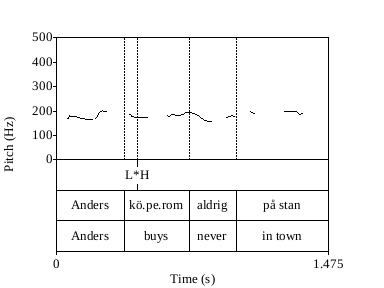
\includegraphics[height=.35\textheight]{figures/erteschik1.png}
\caption{Swedish TU formation, Accent 1 verb \textit{köper} (buy.\textsc{prs)} \textit{+ dom} (them) ‘buys them’.} 
\label{fig:erteschik:1}
\end{figure}

  

 

\begin{figure}
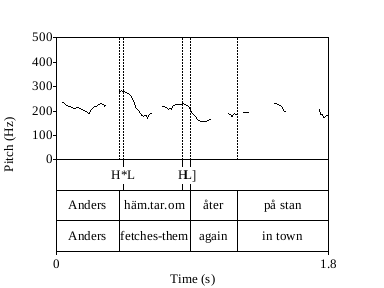
\includegraphics[height=.35\textheight]{figures/erteschik2.png}
\caption{Swedish TU formation, Accent 2 verb \textit{hämtar} (fetch.\textsc{prs}) + \textit{dem} ‘fetches them’}
\label{fig:erteschik:2}
\end{figure}

We suggest that weak pronouns may incorporate in the unit created by the TU, also when the preceding element is an adverb. For example, in \REF{ex:erteschik:1b} \textit{Jag mötte inte honom} (I met him not) ‘I didn’t meet him’, the weak pronoun \textit{honom} ‘him’ is incorporated in the same TU as the preceding adverb \textit{inte} ‘not’. Crucially, this does not mean that the adverb is the host for the pronoun; it is the tonal accent which allows the formation of this prosodic unit. The possibility of incorporating weak object pronouns into a TU is possible only in those varieties of MSc that have TUs, that is those varieties that have tonal accent.

  If our proposal is correct, we predict that the sequence adverb + a weak object pronoun displays a \isi{tone} contour, specified as Accent 1 or Accent 2. More specifically, we predict that an Accent 1 adverb + weak object pronoun will have an Accent 1 contour, and an Accent 2 adverb + weak object  pronoun an Accent 2 contour. To a native speaker’s ear, this seems indeed to be the case in \ili{Swedish}. For example \textit{inte honom} (see \ref{ex:erteschik:1b}) has Accent 2, whereas \textit{faktiskt honom} Accent 1. (The adverb \textit{faktiskt} ‘in fact’ has Accent 1, and the adverb \textit{inte} Accent 2.) 

  The Praat diagrams show adverb + weak pronoun sequences. Recall that the prosodic structure of Accent 1 in \ili{Swedish} is L*H (L\%)  (see (\ref{ex:erteschik:3}) above). This is also what we find for the sequence \textit{åter dom} ‘again them’ in \figref{fig:erteschik:3}.

\begin{figure}
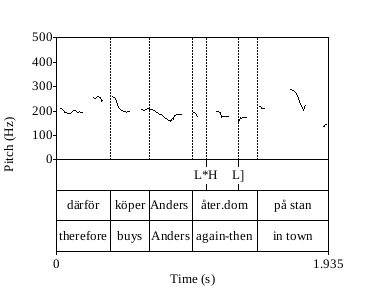
\includegraphics[height=.35\textheight]{figures/erteschik3.png}
\caption{Swedish TU formation, Accent 1 adverb + pronoun → Accent 1}
\label{fig:erteschik:3}
\end{figure}

The prosodic structure of Accent 2 in \ili{Swedish} is H*LH (L\%) (see (\ref{ex:erteschik:3}b) above). This is also what we find for the sequence \textit{aldrig dom} ‘never them’ in \figref{fig:erteschik:4}.

\begin{figure}[H]
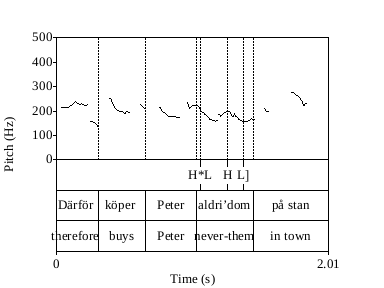
\includegraphics[height=.35\textheight]{figures/erteschik4.png}
\caption{Swedish TU formation, Accent 2 adverb + pronoun → Accent 2}
\label{fig:erteschik:4}
\end{figure}

As we can see, the sequences \textit{åter dem} and \textit{aldrig dem} make up one TU. The \isi{tone}, Accent 1 or Accent 2, is determined by the \isi{tone} of the adverb. This supports our claim that weak object pronouns may form TUs with adverbs.

\ili{Ærø Danish} instantiates another dialect with both tonal distinctions and optional OS and therefore provides a strong case in favor of the current proposal. As pointed out above, tonal distinctions are limited to certain south \ili{Danish} dialects which vary greatly in the way the tones are instantiated. The prediction concerning the particular \isi{tone} to be found on the sequence of adverb(s) + pronoun(s) is again that the \isi{tone} of the unit depends on the \isi{tone} of the first element.

In the Ærø dialect Accent 1 rises until the stressed syllable and then descends, whereas Accent 2 has an initial descending \isi{tone} followed by a rise at the end of the word. The descending \isi{tone} is more pronounced in Accent 1 and the rising \isi{tone} is more pronounced in Accent 2.\footnote{See \citealt{Kroman1947} for an extensive description of tonal accents in this dialect.} This is shown in Figures~\ref{fig:erteschik:5} and \ref{fig:erteschik:6}.

  

 

\begin{figure}
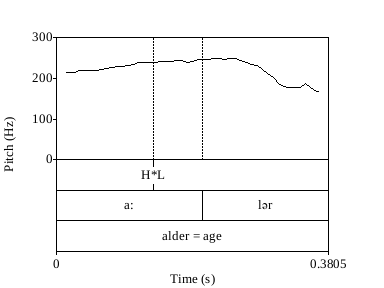
\includegraphics[height=.35\textheight]{figures/erteschik5.png}
\caption{The Ærø dialect, Accent 1 \textit{alder} ‘age’, pronounced \textsuperscript{1}aller.}
\label{fig:erteschik:5}
\end{figure}

  

 

\begin{figure}
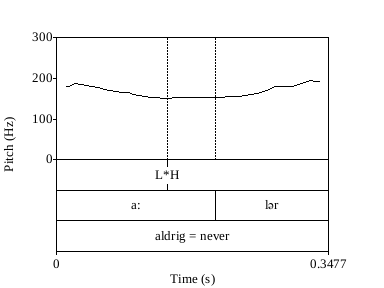
\includegraphics[height=.35\textheight]{figures/erteschik6.png}
\caption{The Ærø dialect, Accent 2 \textit{aldrig} ‘never’, pronounced \textsuperscript{2}aller.} 
\label{fig:erteschik:6}
\end{figure}

\figref{fig:erteschik:7} shows the sequence \textit{så henne} ’saw her’, which has the same prosodic contour as the Accent 1 \textit{alder} ‘age’  in \figref{fig:erteschik:5}.

  

 

\begin{figure}
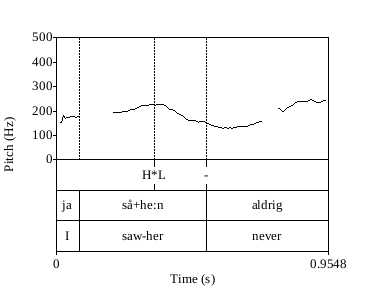
\includegraphics[height=.35\textheight]{figures/erteschik7.png}
\caption{The Ærø dialect, Accent 1 verb + pronoun → Accent 1 TU}
\label{fig:erteschik:7}
\end{figure}

\figref{fig:erteschik:8} shows the sequence \textit{henter dem}, with the Accent 2 verb \textit{henter} (fetch.\textsc{prs}) ‘fetches’ + the pronoun \textit{dem} ‘them’. The sequence \textit{henter dem} ‘fetches them’ has the same prosodic contour as the Accent 2 \textit{aldrig} ‘never’ in \figref{fig:erteschik:5}.

  

 

\begin{figure}
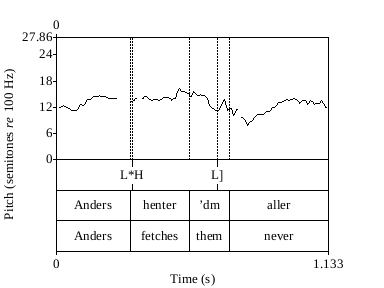
\includegraphics[height=.35\textheight]{figures/erteschik8.png}
\caption{The Ærø dialect, Accent 2 verb + pronoun → Accent 2 TU}
\label{fig:erteschik:8}
\end{figure}

Let us now consider the sequence adverb + pronoun, in other words cases of non-shift in the Ærø dialect. The prediction is that the result will be the same as in the corresponding sentences in \ili{Swedish}, namely that adverb + weak pronoun will form a TU. Consider first the sequence \textit{lige} ‘just’ + \textit{dem} ‘them’. The adverb \textit{lige} ‘just’ is an Accent 1 adverb (see \figref{fig:erteschik:9}).


  

 


\begin{figure}
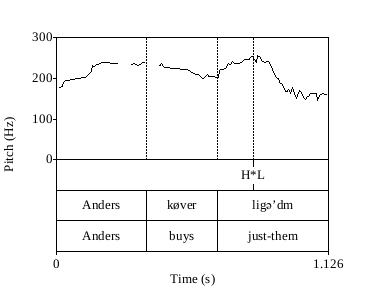
\includegraphics[height=.35\textheight]{figures/erteschik9.png}
\caption{The Ærø dialect, Accent 1 adverb + pronoun → Accent 1 TU}
\label{fig:erteschik:9}
\end{figure}

We also predict that an Accent 2 adverb + pronoun will give rise to an Accent 2 TU (see \figref{fig:erteschik:10}).

  

 

\begin{figure}
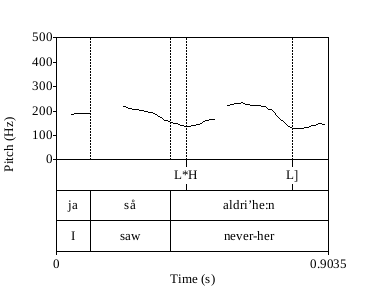
\includegraphics[height=.35\textheight]{figures/erteschik10.png}
\caption{The Ærø dialect, Accent 2 adverb \textit{aldrig} ‘never’  + pronoun → Accent 2 TU}
\label{fig:erteschik:10}
\end{figure}

As we have seen, the prediction is supported: the sequence adverb + weak pronoun forms a TU, in the same way as in \ili{Swedish}.

As an experiment, three Ærø informants were asked to repeat sentences where the object pronoun had undergone OS. All three informants reversed most of the test sentences with OS and rendered them with the object following the adverb. This was consistently the case with the adverb ‘not’ (\textit{ikke} in standard \ili{Danish}, \textit{it} in the Ærø dialect) but not with the longer adverbs, e.g. \textit{aldrig} ‘never’. As will be shown below for Falster-\ili{Danish}, monosyllabic adverbs, or cases in which adverbs become monosyllabic due to apocope, must cliticize in certain dialects rendering the order V-Adverb-pronoun. This is preferred in Ærø-\ili{Danish}, but not required.

\section{Potential counterexamples: Norwegian Vesttrødersk, Danish Lolland-Falster and Fenno-Swedish}\label{sec:erteschik:5}

The Lolland-Falster dialect has been claimed to have optional Object Shift, i.e., to allow the order adverb + weak pronoun even though tonal distinctions are absent from these dialects. \ili{Fenno-Swedish} poses another problem: OS has been claimed to be absent in this dialect – even though there is no tonal accent distinction. 

Our prosodic analysis of object-shifted and non-object-shifted sentences in \ili{Swedish} and Ærøese shows that the weak pronouns in both orders are tonally incorporated into their hosts. We argue that the formation of a TU consisting of adverb + pronoun requires a tonal accent but that the existence of tonal accent does not necessarily {force} optional OS. This is attested in \ili{Norwegian}. In Vesttrødersk (=Nordmørsk), for example, Object Shift is strongly preferred. In the dialect of Trødersk spoken in most parts of Trøndelag (e.g., Trondheim), however, \isi{negation} undergoes apocope (\textit{ikkje} → \textit{itj}) resulting in a monosyllabic \isi{clitic}. In this dialect and with this adverb, pronouncing the pronoun in situ is strongly preferred. If we assume that the word order~\textit{såg} \textit{itj'n}~(saw=not=it) ‘didn’t see it’ is due to the \isi{clitic} nature of the negative adverb, we have an explanation of the difference between these two dialects and the limitation of the phenomenon to the \isi{clitic} adverb. We recorded both these dialects and verified these facts.

This phenomenon in \ili{Norwegian} gave us the inspiration for an explanation of the seeming exceptional properties of Lolland-Falster \ili{Danish}. As it turns out one of the properties of the Lolland-Falster dialect is that it has apocope and that \isi{negation} is monosyllabic. In order to verify that this is what is going on, recordings were made of two speakers of the Falster dialect in April 2015. (It should be noted that speakers of the dialect are no longer easy to find and can be found only among the older generation). It turned out that our hypothesis was correct: both speakers had obligatory Object Shift, as in standard \ili{Danish}, for all adverbs except for the \isi{clitic} adverbs \textit{ik} ‘not’ and \textit{jo} ‘as presumed’. The recordings clearly show \isi{clitic} clusters for these adverbs as illustrated in \figref{fig:erteschik:11}. Note that the weak element is an adverb, \textit{her} ‘here’. However, the weak adverbs \textit{der} ‘there’ and \textit{her} ‘here’ undergo OS in \ili{Danish}. 

  

 
\begin{figure}
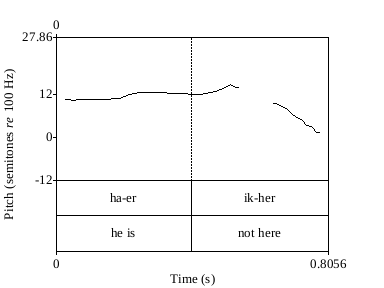
\includegraphics[height=.35\textheight]{figures/erteschik11.png}
\caption{The Lolland-Falster dialect, the negation \textit{ik} + \textit{her} ‘here’}
\label{fig:erteschik:11}
\end{figure}

Interestingly the following example was produced spontaneously:

\ea%7
\label{ex:erteschik:7}
\gll Jeg   kender+jo+ik+(h)am. \\
     I     know=\textsc{jo}=\textsc{neg}=him\\
    \glt ’I don’t know him.’
    \z

We were happy to conclude that this \ili{Danish} dialect does not, in fact, provide a problem for our thesis. Falster \ili{Danish} has obligatory Object Shift, as we predict for a dialect without tonal distinctions. The cases of in-situ weak pronouns are limited to \isi{clitic} adverbs, which cliticize into the verbs, themselves forming a clitic-cluster with the following weak adverbs. We were surprised to discover that \citegen{Pedersen1993} claim that OS is optional in the Lolland-Falster dialect was in fact limited to the negative adverb.

\ili{Fenno-Swedish} presents a different problem since OS is not available \citep[72]{Bergroth1917}. \ili{Fenno-Swedish} differs significantly from Standard \ili{Swedish} in not having tonal distinctions, contra our prediction. \citet[17]{Kiparsky2008} includes pronouns in his list of function words with short stressed syllables in Helsinki \ili{Swedish}. This indicates that pronouns in this dialect are not prosodically weak. If this is indeed the case, our prediction does not apply to \ili{Fenno-Swedish} since this dialect would not require incorporation of weak pronouns into the adverb, and it is only such incorporation which requires the formation of a TU. The lack of tonal distinctions in \ili{Fenno-Swedish} would then no longer be a problem. In May 2015, three speakers of \ili{Fenno-Swedish} from Helsinki were recorded and the findings were that the given pronouns were not reduced and definitely not incorporated in the preceding adverbs. 

More investigation is needed, of course, but initial data indicates that neither Falster \ili{Danish} nor \ili{Fenno-Swedish} contradict our accent-based analysis of the optionality of OS. 

\section{Architectural implications}\label{sec:erteschik:6}

In previous work we have each independently examined the phonological properties of OS. Here we focus on the optionality of Object Shift and show that leaving the weak pronoun in situ is licensed by tonal accent, further strengthening our argument for the claim that OS is determined by PF. Leaving OS in MSc to phonology allows for at least some cases of word order to be determined in the phonology. Since the full range of properties of OS has not to-date been given a satisfactory syntactic account, this is a good result and falls nicely within the proposal in \citet{Berwick2011}, that displacement is constrained by the syntactic computational system, and the PF externalization system is responsible for at least microvariation. One implementation of this approach would have OS operate in the computational system and have PF act as a filter on its output. The only “advantage” of this approach is to exclude movement from PF in the case of OS. Another would be to have the position of the object fully determined by phonological processes and constraints. This implementation raises questions concerning what reordering in phonology would look like, and what other word order phenomena belong at PF.

\section{Summary}

We have come a long way in verifying our initial hypothesis concerning the connection between word order and prosody. In particular, we have found that the order adverb + weak pronoun forms a Tonal\is{tonal unit} Unit licensed by a single unifying accent\largerpage which is not limited to syntactic constituents.

The three seeming exceptions to this generalization, Vesttrødersk \ili{Norwegian}, Lolland-Falster \ili{Danish}, and \ili{Fenno-Swedish} have been shown to receive explanations following from the particular prosodic properties of each of these dialects: apocope in the former two, and the lack of reduction of weak pronouns in the latter.

In addition to explaining the variation in Object Shift in the various dialects we also provide a deeper understanding of the prosodic properties of the dialects in {question} as well as furthering the understanding of the prosody/word-order interface in general.

\section*{Acknowledgements}

First and foremost we want to thank Anders Holmberg for having inspired us to write this paper, and also for being inspirational over the years – in many different areas of linguistics. Anders’ greatness stems from a mind open to new ideas, curiosity and an eye for small details as well as broad generalizations. Thank you, Anders! 

The research for this work was funded by the Israel Science Foundation Grant No. 302/13. We are indebted to Björn Koenlein for valuable assistance in the interpretation of the prosodic data. We would also like to thank an anonymous reviewer for valuable comments. Earlier versions of this paper have been presented at {Hebrew} University, Jerusalem; Tel Aviv University; the 25th {Scandinavian} Conference of Linguistics, Reykjavik, May 2013; and at the Grammar seminar, Centre of Languages and Literature, Lund University, March 2014. We would like to thank the participants at those occasions for valuable input. All remaining errors and inadequacies are our own.
{\sloppy
\printbibliography[heading=subbibliography,notkeyword=this]
}
\end{document}